%%%%%%%%%%%%%%%%%%%%%%%%%%%%%%%%%%%%%%%%%%%%%%
%                insertmeeting
% 1) Title (something creative & funny?)
% 2) Date (MM/DD/YYYY)
% 3) Location (ex. Hagerty High School)
% 4) People/Committees Present 
% 5) Picture 
% 6) Start Time & Stop Time (ex. 12:30AM to 4:30PM)
%%%%%%%%%%%%%%%%%%%%%%%%%%%%%%%%%%%%%%%%%%%%%%
\insertmeeting 
  {Revision Race} 
  {11/28/21}
  {Hagerty High School}
  {James, Nathan, Ritam}
  {Images/RobotPics/robot.jpg}
  {2:30 - 4:30}
  
\hhscommittee{Hardware}
\noindent\hfil\rule{\textwidth}{.4pt}\hfil
\subsubsection*{Goals}
\begin{itemize}
    \item Make several changes to carbon fiber sides
    \item Use variables to make changes to cad easier


\end{itemize} 

\noindent\hfil\rule{\textwidth}{.4pt}\hfil

\subsubsection*{Accomplishments}

Although we believed the carbon fiber sides and their molds to be complete after yesterday’s meeting, there are a couple changes we wanted to make. The first is to extend the length of the plates all the way to the back of the robot. This will allow us to connect the back stop plate to the carbon fiber plates to increase strength. Making this change seemed like it would be easy, but because we used the project tool instead of using variables for many of the components, several parts of the model broke while trying to reposition the side plates. This meant that we spent lots of time remaking all of the parts that broke in CAD, rather than spending time improving or printing the model. Another problem we realized was the dimensions of the sideplates. We hadn’t left enough vertical room before curving the plates inward for our numbers to fit. Although we could just make the numbers out of a flexible material and allowed them to curve with the sides, when checking the game manual, we found that this might be illegal because the 2 sets of numbers must be facing in completely opposite directions. Because of this, we planned on simply changing the dimensions to move the curve higher up, but soon found the same issue that had arisen when trying to extend the plate to the back of the robot, where many of the other parts had errors because their references had changed. After fighting with the CAD for a while, we started to think about how we could fix these issues by using more variables which don’t require references to work like the project tool does. When we weighed our options we decided that in case of any other changes that might need to be made, we would redesign the side plates and mold to be able to change without creating errors. Because we had already made the side plates once, recreating them would go a bit quicker and we would already have the foresight to create the design to be parametric and easy to change.
Getting started right away, we created some of the major variables that we knew we might want to change at some point in the future. These variables, and the ones we added later, would be the primary way to change any detail about the side plates (Figure \ref{fig:112821_1}). Working with these variables and using more constraints, we recreated the side plates and their molds, creating an end result that appears very similar but is much more future-proof (Figure \ref{fig:112821_2}). The variability of the redesigned side plates paid off almost immediately as we were able to easily change the distance between the sides at the top of each plate. this change, although simple, would have caused errors on almost every feature of the old design, but with the new parametric variable system utilized on the new side plates was changed simply by editing the variable top dist, which automatically changed every part of the design accordingly using mathematical expressions we wrote into the variable and other variables inheriting from it.

 

\begin{figure}[ht]
\centering
\begin{minipage}[b]{.48\textwidth}
  \centering
  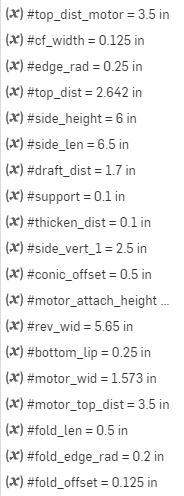
\includegraphics[width=0.95\textwidth]{Meetings/November/11-28-21/11-28-21_CAD_Figure1 - Nathan Forrer.JPG}
  \caption{Our CAD variables for the sideplates}
  \label{fig:112821_1}
\end{minipage}%
\hfill%
\begin{minipage}[b]{.48\textwidth}
  \centering
  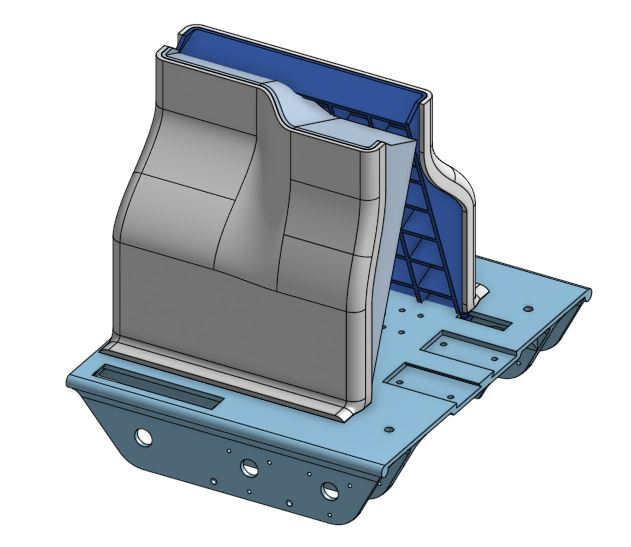
\includegraphics[width=0.95\textwidth]{Meetings/November/11-28-21/11-28-21_CAD_Figure2 - Nathan Forrer.JPG}
  \caption{The redesigned CAD using our variables}
  \label{fig:112821_2}
\end{minipage}
\end{figure}


\whatsnext{
\begin{itemize}
    \item 3D print carbon fiber side molds
    \item Use mold to create sides out of carbon fiber 

\end{itemize} 
}

